\documentclass[]{tufte-handout}
\usepackage{amsmath,amssymb,amsthm}
\usepackage[pdftex]{graphicx}

\title{COMP 161 --- Lecture Notes 15 \\ Complexity and Big-O}
\date{}

\newtheorem{define}{Definition}
\newtheorem{theorem}{Theorem}

\begin{document}
\maketitle

\begin{abstract}
In these lecture notes we look at algorithm complexity and the use of Big-O notation to express complexity classes.
\end{abstract}

\section{Efficiency, Complexity, and Computational Resources}

Being efficient means optimizing the use of one or more resources.  A fuel efficient car will travel far while minimizing the consumption of fuel. This means the ratio of miles traveled per gallon of fuel is high relative to a less efficient vehicle\sidenote{conversely the ratio of gallons consumed per mile is lower}.  When comparing cars for fuel efficiency we tend to look at things like the expected miles per gallon or perhaps the highest achievable miles per gallon. In both cases, we're operating the car not under a guarantee of peak efficiency but with an understanding that we can expect a certain level of efficiency when driving. In short, we understand that manufactures typically provide us with theoretically achievable efficiency for our vehicle and that in practice, mileage may vary.

Of course efficiency is not a singular measure. It is relative to the consumption of a specific resource.  Perhaps the consumption of fuel is not your concern, but time is.  A time efficient car would exhibit a higher acceleration rate and/or top speed.  We typically expect that this increased time efficiency came at the cost of fuel efficiency. So not only is efficiency subjective, but the overall efficiency of a vehicle involves trade offs.  Less time means more fuel, less fuel means more time.

\subsection{Complexity}

Enough about cars. What about computers and computation? The most discussed and emphasized computational resource around is \textsc{time}. Time efficient computations take less time.  We then tend to look at other resources in terms of their relationship with time. By increasing the \textsc{space}\sidenote{memory} needs of a computation we can often decrease the \textit{time} needs.  Conversely, decreasing space often requires increased time. In this way space might be viewed as the fuel of computation. There are still more resources used in computation. When we get into parallel computation, we start to think about things like \textsc{communication} as a resource.  The less computers working in parallel have to communicate, the less time they need and vice versa.

\textsc{Complexity Theory} is the branch of theoretical computer science in which problems are classified by the resource needs of their solutions.  Go look at the documentation for C++ library procedures and class methods on cplusplus.com and you'll see a section title \textit{Complexity}.  This is exactly the complexity theoretic view of the efficiency of that procedure. It provides the programmer with a broad classification of the efficiency of the procedure in favor of a fine-grained view. From the programmer's perspective, complexity measures of efficiency provide you with an expectation of efficiency in much the same way that a car manufacture's reported miles per gallon does for fuel efficiency. The specifics of your usage of a procedure, the actual inputs, the actual state of the system, will have an impact on the time needed but the complexity provides some general guarantees.

Unless otherwise specified, complexity classifications are based on the \textsc{worst case} resource needs of the procedure. The worst and best case are often generated by a very specific variation of the input and it's easier to be concrete about their resource needs. For example, the basic search procedure's best case is when the item we're looking for is the first item we look at and it's worst case is when it's the last. The average case is much less specific; it's when the item we're looking for is neither the first nor the last.  Given a choice between best case and worst case thinking, we err on the side of worst case.  Knowing that your program needs at most some amount of time means that on average we can can expect that efficiency or better.  This \textsc{upper bound} on the resource needs is ultimately more useful to the programmer than the \textit{lower bound} offered by the best case.

Complexity theory is carried out in a machine and language agnostic fashion. We measure time by counting basic operations, not by the clock. We measure space sometimes by bits and bytes but sometimes by abstract, discrete units of data. By classifying procedures in this way we are able to rule out the language used and the machine executing the code and instead focus on some underlying abstract model of computation. In doing so, the assessment of a procedure's complexity becomes an assessment of the underlying \textit{algorithm} and not the actual implementation. As a discipline of study, complexity theory is smack dab at the intersection of mathematics and computer science\sidenote{The work itself is done in mathematics where the objects of study are those of computer science. The distinction between the two disciplines gets awful blurry in this realm}. For our purposes, we simply with to apply the basic principles, broad categorization of program efficiency based on the the expected worst case performance of the procedures, to program design and evaluation.

\section{ Big-O }

There is a precise mathematical tool call \textsc{Big-O notation} that we can use to express the relationship we're looking for when expressing procedure complexity.
\begin{define}
Let the functions $f$ and $g$ be functions for positive integers.  Then the function $f$ is \textit{on the order of} $g$ if there exists constants $n_0 \geq 0 $ and $\alpha$ such that for all $n 	\geq n_0$
\[
f(n) \leq \alpha g(n)
\]
We write this as $f(n) = O(g(n))$, or sometimes just $f = O(g)$,\sidenote{O is uppercase letter o, not the number zero} and often say ``$f$ is Big-O of $g$'' as opposed to ``$f$ is on the order of $g$''.
\label{def:bigO}
\end{define}

Let's pick this apart so that we understand what saying $f = O(g)$ really means. First notice it's clearly an upperbound relationship. The value $\alpha g(n)$ is at least as big as $f(n)$. The $\alpha$ term is allowing us to focus not on the specific value of $g(n)$ as our bound but nearly any multiple of $g(n)$.  We're more or less saying that ``$f(n)$ is no larger than some multiple of $g(n)$''.  Finally, by throwing in $n_0$ we're emphasizing ``larger'' values of $n$ for whatever large means to us. Putting this all together we see that $f = O(g)$ really means:
\begin{quote}
For all $n$ past some point\sidenote{$n_0$}, we can draw some multiple\sidenote{$\alpha$} of $g$ on or above $f$
\end{quote}
The notion of Big-O gives us the right mixture of specificity and flexibility for capturing complexity and complexity classes.

In future courses you'll explore this formalism in more depth. Right now we want to learn some basic rules and relationships that follow such that we understand how Big-O communicates complexity classes. There are three basic consequences of definition~\ref{def:bigO} that are essential to working with Big-O in both a formal and informal manner. I'll state them formally and then provide some insight as to why they are so essential to complexity analysis.

The order of a sum is the sum of the orders.
\begin{theorem}
Let $f$ and $g$ be functions over the positive integers. Then,
\[
O(f + g) = O(f) + O(g)
\]
\label{th:sum}
\end{theorem}
All procedures can be broken down into a series of steps. This theorem (\ref{th:sum}) tells us that it is enough to know the order of each step. This let's us greatly simplify complexity analysis by doing it piecewise rather than on the whole.

We have two properties that deal with produces and Big-O. The order of a product is the product of the orders.
\begin{theorem}
Let $f$ and $g$ be functions over the positive integers. Then,
\[
O(fg) = O(f)O(g)
\]
\label{th:mult}
\end{theorem}
The order of a function is invariant under multiplication by a constant.
\begin{theorem}
Let $f$ and $g$ be functions over the positive integers. Then for all real-values $\alpha$,
\[
O(\alpha g) = O(g)
\]
\label{th:constmult}
\end{theorem}
A great number of procedures involve repetition and repetition induces a product.\sidenote{Repeating $k$ operators $t$ times takes $tk$ operations in total}. When the repetition is done a fixed number of times, then theorem (\ref{th:constmult}) tells us that the order of the repetition is the same as the the order of the thing being repeated. Similarly, if we repeat some fixed, constant amount of work, some function of our input size number of times, then theorem (\ref{th:constmult}) tells us that the order of the repetition is the order of them number of function that determines the number of repetitions. If, however, the repetition and the work are both functions of our input size, then theorem (\ref{th:mult}) tells us that we can at least analyze the order of the repetition and the order of the repeated work in parts but cannot really simplify to one order or the other.


Using Big-O we can establish a strict ordering of some functions. This will be true of the functions on which we'll base our complexity classes. It turns out that larger orders dominate smaller orders.
\begin{theorem}
For functions $f$ and $g$. If $O(f) < O(g)$, then
\[
O(f) + O(g) = O(g)
\]
\label{th:order}
\end{theorem}
Once again, sums arise from the discrete steps of a computation. When one step requires an order of magnitude more computation than another step, then that step dominates the total running time of the computation to the point that the whole computation behaves as if it were only of that larger complexity class. What Theorem~\ref{th:order} lets us do is focus solely on the critical steps that account for most of the work.\sidenote{I tend to think of this rule in terms of spending money. If you're paying thousands of dollars for something, then adding on tens of dollars doesn't really change the big picture-- you're paying thousands of dollars for something.If you're paying \$5000, then you'll probably also pay $5050$}.

Hopefully you're picking up on the fact that these rules have close ties to the constructs of programs. The step-wise nature of induces sums in our time complexity functions and those sums can be more easily managed using theorem (\ref{th:sum}). Repetition induces products in our time complexity functions and those produces can be managed with theorem (\ref{th:mult}) and (\ref{th:constmult}). The analysis of conditionals is simplified by the fact that we're only concerned with the worst case. If we know which branch has the highest order, then we can focus on that branch.

\section{Some Complexity Classes}

Remember our intended use for Big-O notation is the classification of the (time) complexity of procedures in order to address the questions like whether or not one procedure is more or less complex than another or if a given procedure is too complex to be usable in practice. A large majority of the procedures we encounter have a time function which is on the order of one of the following functions. These functions, in turn, establish a clear ordering of classes.

\begin{enumerate}
\item \textsc{Constant} \\
 If the complexity function $f$ is constant, i.e. $f(n) = c$ for some fixed value $c$,  then we say $f = O(1)$.

\item \textsc{Logarithmic} \\
 If the complexity function $f$ is  logarithmic, i.e. $f(n) = \log_b n$, then we say $f = O(\log n)$. Notice that we leave off the base of the logarithm. It can be shown that the base of the logarithm actually doesn't matter in Big-O notation\sidenote{$O(\log_a n) = O(\log_b n)$ for all $a$ and $b$} so we typically use 2. You'll often see $\log_2$ written as $\lg$

\item \textsc{Linear} \\
 If the complexity function $f$ is linear, i.e. $f(n) = n$, then we say $f = O(n)$.

\item \textsc{Linearithmic}\sidenote{a blend of linear and logarithmic} \\
 If the complexity function $f$ is the product of linear and logarithmic function, i.e. $f(n) = n\log n$, then we say $f = O(n\log n)$.

\item \textsc{Quadratic} \\
 If the complexity function $f$ is a quadratic function, i.e. $f(n) = n^2$, then we say $f = O(n^2)$.

\item \textsc{Cubic} \\
If the complexity function $f$ is a cubic function, i.e. $f(n) = n^3$, then we say $f = O(n^3)$.

\item \textsc{Exponential} \\
If the complexity function $f$ is a exponential for some constant $c>1$, i.e. $f(n) = c^n$. We express this as  $f = O(c^n)$.

\item \textsc{Factorial} \\
If the complexity function $f$ is the factorial, i.e. $f(n) = n!$, then we say $f = O(n!)$.
\end{enumerate}

Within each class there is an awful lot of nuance. For example, pick any time function where $\mathcal{f}(n)= an + b$, then $f = O(n)$. As you may remember from math class, the larger the value of $a$ the greater the slope of the line and the faster it grows. Big-O notation completely ignores this reality and instead groups all lines together. That's ok, the point of Big-O and complexity classes are not specific, nuanced details, but big picture, order of magnitude details.

The complexity classes we use are represented by basic, well understood functions for which there is a strict least to greatest growth rate order.
\[
O(1) < O(\log n) < O(n) < O(n \log n) < O(n^2) < O(n^3) < O(c^n) < O(n!)
\]
If you have two different procedures that solve the same problem and one has work $O(n)$ and the other has work $O(n \log n)$, then you know the first, the linear work option, is \textit{a whole order of magnitude better} than the later. This is what we get from Big-O and complexity classes. We get the ability to partition the infinite world of procedures into simple efficiency complexity classes that allow us to quickly and easily identify order of magnitude differences.

On the practical side of things, we can also quickly identify when a procedure will be impractical. Computer science has drawn a line in the sand at \textsc{Polynomial complexity} such that any complexity class that is a polynomial or better is theoretically efficient. This includes everything on our list but $O(2^n)$ and $O(n!)$. It turns out that this somewhat arbitrary choice works pretty well in practice. However, cubic and quadratic functions do grow pretty quickly and can easily be impractical for even modest $n$.  Superlinear or better is almost always practical, even for very large $n$.  You'll get a very real sense of this in your final project, but let's look at some numbers to get you thinking.


First lets look at how each function grows as $n$ grows.
\begin{figure}
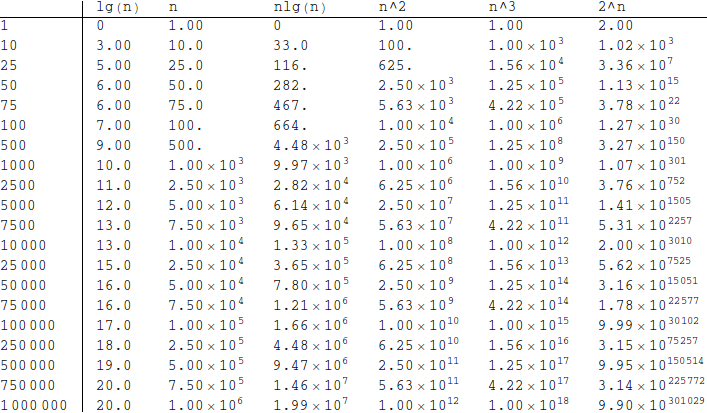
\includegraphics[scale=0.45]{nvals.png}
\caption{The value of key complexity class functions for increasing values of $n$}
\end{figure}

Now imagine you have a computer that performs 1 operation every nanoseconds\sidenote{also known as a 1 Gigaflop GFLOP computerThis is actually fairly modest by today's standards. Your average laptop can probably do two to five times better than this.} Then, we can attach some time amounts to these complexity classes.
\begin{figure}
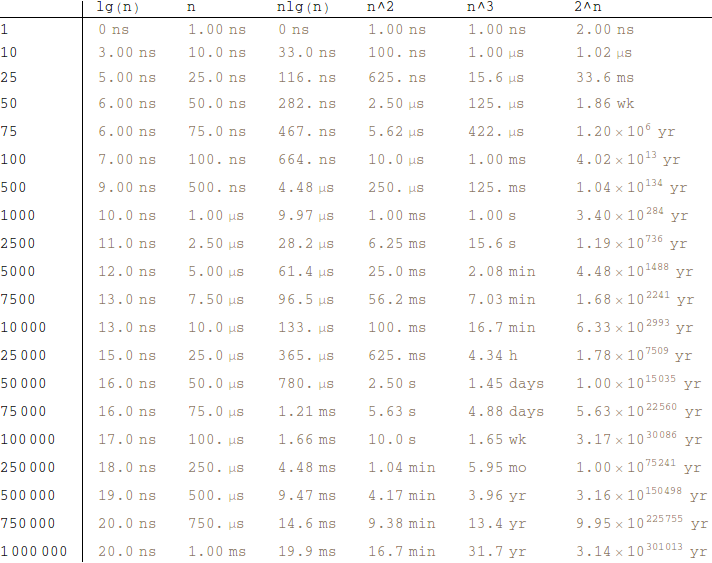
\includegraphics[scale=0.45]{timevals.png}
\caption{The time needed to compute key complexity class functions at 1GFLOP}
\end{figure}





\end{document}
